% Author: Seongjin Lee 
% Hanyang University, Seoul, Korea 
% esos.hanyang.ac.kr 
% 2016-09-20
% note: some slides are adopted from  \url{www.cs.stevens.edu/~jschauma/631A/}
% https://github.com/resourceful/lecture_sysprog/

\documentclass[newPxFont,sthlmFooter,nooffset]{beamer}
\usepackage{kotex}
\usepackage{blindtext}
\usepackage{framed, color}
\usepackage{mdframed}
\usepackage{setspace}
\definecolor{shadecolor}{rgb}{0.1,0.1,0.1}
%\usetheme{sthlm}
\usepackage{../beamer_template/beamerthemesthlm}

\hypersetup{pdfauthor={Seongjin Lee (nyg0813@gmail.com)},
            pdfsubject={Lecture Note: System Programming},
            pdfkeywords={Lecture Note, System Programming, class, undergraduate},
            pdfcreator={Yeonjin Noh}}

%\setbeamertemplate{footline}[text line]{%
%    \parbox{\linewidth}{\vspace*{-8pt} \insertsectionhead  \hfill\insertshortauthor\hfill\insertpagenumber}}
%\setbeamertemplate{navigation symbols}{}



\title{System Programming}
\subtitle{Topic 5: Ctags}
\author[YJN]{Yeonjin Noh}
\institute{\href{mailto:nyg0813@gmail.com}{nyg0813@gmail.com}\\\url{http://esos.hanyang.ac.kr}\\Esos Lab. Hanyang University}
\date{2016-09-27} 

\begin{document}



\frame[plain]{\titlepage} 

\frame{\frametitle{Table of contents}\tableofcontents} 


%---------------------------------------------------------

\begin{frame}[t]
  \frametitle{Introduction}
\begin{block}{Ctags란?}
\medskip
프로그래밍 소스코드에서 함수의 정의, 매크로 선언들과 소스 코드의 태그들의 \textbf{Database}(\textbf{tags file})를 생성하는 Unix 명령어
\end{block}
\smallskip
다시말해, \\
\bigskip
소스코드 내부의 함수 및 변수의 위치를 쉽게 인식 할 수 있도록\\ 
\begin{Large}
\textcolor{red}{\textbf{인덱스}(\textbf{index})}
\end{Large}를 만드는 명령어라 정의할 수 있다.
\end{frame}
\begin{frame}[t]
  \frametitle{Ctags의 장점}
\begin{itemize}
\item 함수의 검색 및 함수가 정의된 곳으로 이동이 가능
\item 커널 코드와 같이 큰 규모의 프로젝트의 소스를 분석할 때 유용
\item Vim 및 emacs와 호환 가능
\end{itemize}
\end{frame}
\section{Ctags 환경설정 및 사용법}
\begin{frame}[containsverbatim, t]
  \frametitle{Ctags 설치}
먼저 Ctags를 설치하기 전, 
\begin{mdframed}[backgroundcolor=lightgray,hidealllines=true]
\texttt{\textcolor[rgb]{0,0,0}{\$ ctags -help}}
\end{mdframed}
\bigskip
명령어로 Ctags가 설치되었는지 확인하고, 없다면 아래와 같이 명령어를 입력한다.
\begin{mdframed}[backgroundcolor=lightgray,hidealllines=true]
\texttt{\textcolor[rgb]{0,0,0}{\$ sudo apt-get install ctags}}
\end{mdframed}
\bigskip
\end{frame}

\begin{frame}[containsverbatim,t]
  \frametitle{tags 파일 생성(Skip)}
Ctags를 사용하기 위해서는 `tags 파일'을 생성할 필요가 있다.\\
`tags 파일'을 생성하기 위해서는 분석을 원하는 폴더로 이동한 후 아래의 명령을 입력한다.
\begin{mdframed}[backgroundcolor=lightgray,hidealllines=true]
\texttt{\textcolor[rgb]{0,0,0}{\$ ctags -R}}
\end{mdframed}
\bigskip
생성된 tags 파일은 \texttt{ls} 명령어를 통해 다음과 같이 확인할 수 있다.\\
\begin{figure}[h]
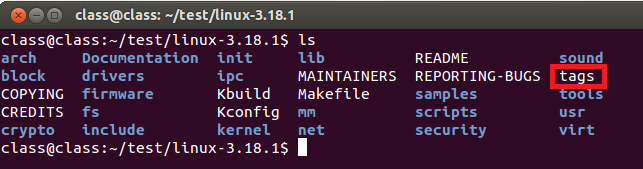
\includegraphics[width=0.98\linewidth]{./figure/tags.png}
\end{figure}
\end{frame}

\begin{frame}[containsverbatim,t]
  \frametitle{tags 파일 복사(Skip)}
Ctags에서 생성한 tags 파일은 절대경로가 아닌 상대경로이기 때문에, 기존에 생성된 tags 파일을 복사하거나 이동시켜서 사용할 수 있다.
\\아래의 명령어를 통해 `tags파일'을 커널코드로 복사한다.
\begin{mdframed}[backgroundcolor=lightgray,hidealllines=true]
\texttt{\textcolor[rgb]{0,0,0}{\$ cp ../codes/tags /'linux소스 코드 경로'/}}
\end{mdframed}
\bigskip
복사된 tags 파일은 \texttt{ls} 명령어를 통해 다음과 같이 확인할 수 있다.\\
\begin{figure}[h]
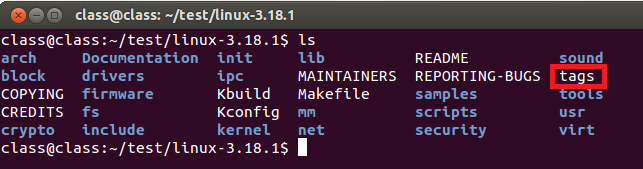
\includegraphics[width=0.98\linewidth]{./figure/tags.png}
\end{figure}
\end{frame}

\begin{frame}[containsverbatim,t]
  \frametitle{tags 파일 열기}
\begin{mdframed}[backgroundcolor=lightgray,hidealllines=true]
\texttt{\textcolor[rgb]{0,0,0}{\$ vi tags}}
\end{mdframed}
\bigskip
위 명령어를 통해 tags 파일을 열어보면, tags 파일은 아래 그림과 같은 구성을 가진다. 
\smallskip
\begin{figure}[h]
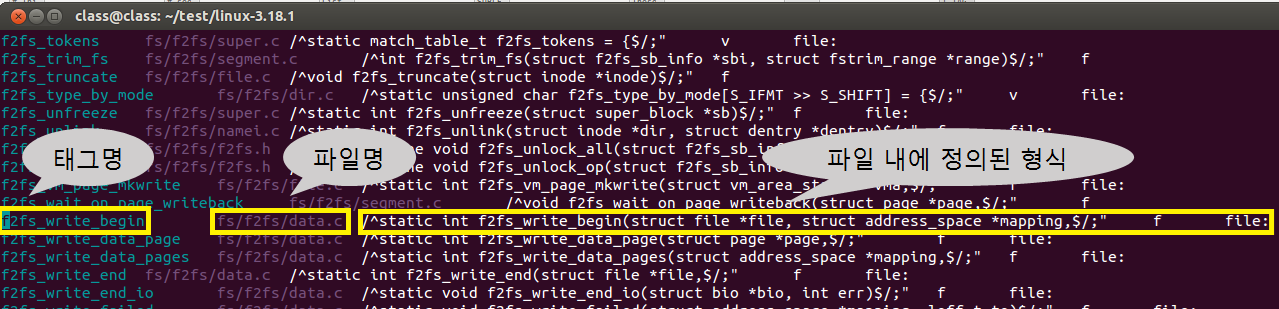
\includegraphics[width=0.98\linewidth]{./figure/tagsinside.png}
\end{figure}
이를 통해 각 함수, 변수에 따라 태그가 생성된 것을 알 수 있다.
\end{frame}

\begin{frame}[containsverbatim,t]
  \frametitle{Ctags 사용법}
\begin{footnotesize}
\textbf{태그 파일을 연 상태}에서 vi를 command line 모드로 변경하고,
\begin{mdframed}[backgroundcolor=lightgray,hidealllines=true]
\texttt{\textcolor[rgb]{0,0,0}{:tj `함수(tag명)'}}
\end{mdframed}
\bigskip
명령어를 입력하여 원하는 함수 및 변수의 위치로 이동할 수 있다. 만약 검색된 태그가 여러개인 경우에는 태그의 목록을 아래 그림과 같이 출력한다.\\
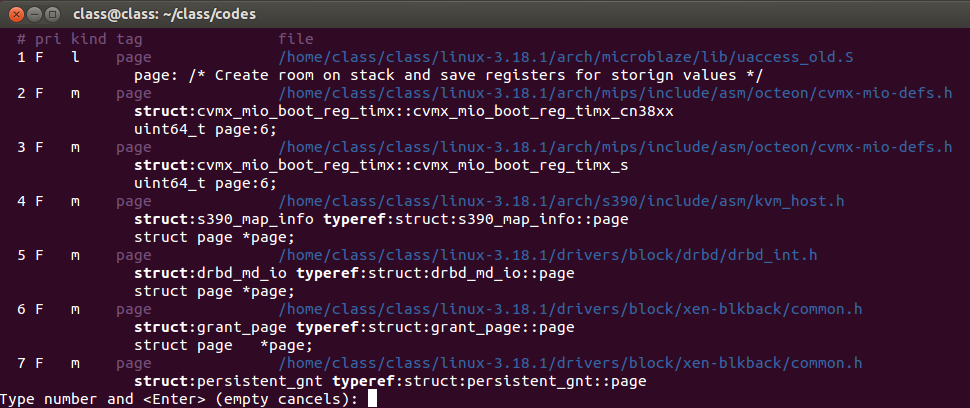
\includegraphics[width=0.8\linewidth]{./figure/ts.png}
\\
다음 태그로 이동은 \texttt{:tn}을 사용하며, \texttt{:ta}는 첫번째 태그의 위치로 즉시 이동한다.
\\
이 외에도, 변수나 함수 위에서 \textbf{\texttt{`Ctrl + ]'}}를 입력하면 함수의 위치로 즉시 이동할 수 있다.
\end{footnotesize}
\end{frame}
\begin{frame}[containsverbatim,t]
  \frametitle{Ctags 사용법}
\begin{mdframed}[backgroundcolor=lightgray,hidealllines=true]
\texttt{\textcolor[rgb]{0,0,0}{:tp}}
\end{mdframed}
\bigskip
혹은\\
\begin{mdframed}[backgroundcolor=lightgray,hidealllines=true]
\texttt{\textcolor[rgb]{0,0,0}{:po}}
\end{mdframed}
\bigskip
명령어를 통해 이전 태그로 돌아갈 수 있으며, \texttt{:tp}나 \texttt{:po} 대신 \textbf{\texttt{`Ctrl + t'}}를 사용하여 즉시 전 태그로 돌아갈 수도 있다.
\end{frame}

\begin{frame}[containsverbatim,t]
  \frametitle{Ctags 사용법}
또한, \textbf{태그 파일을 연 상태}에서,
\begin{mdframed}[backgroundcolor=lightgray,hidealllines=true]
\texttt{\textcolor[rgb]{0,0,0}{:stj `함수(tag명)'}}
\end{mdframed}
\bigskip
명령어를 입력하면 아래와 같이 분할된 창에서 태그를 볼수 있다.
\smallskip
\begin{figure}[h]
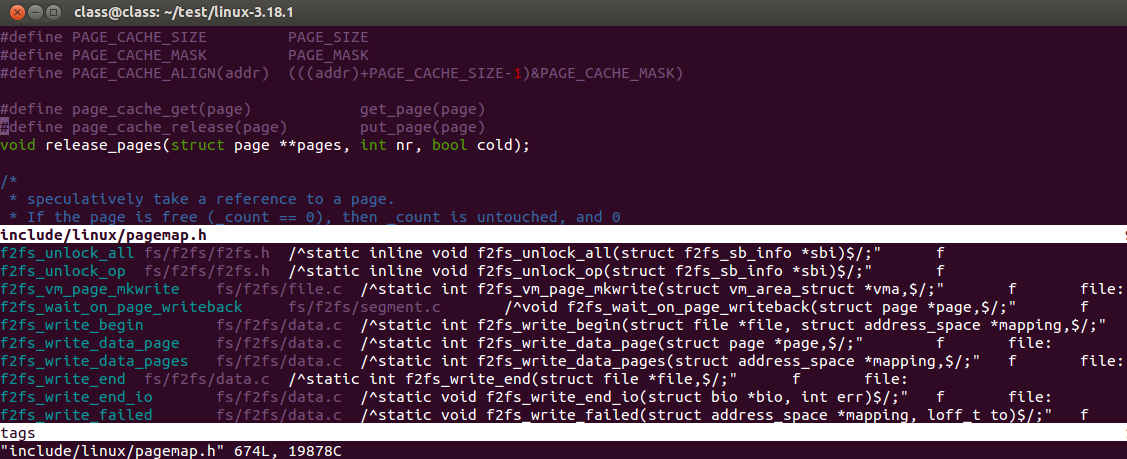
\includegraphics[width=0.98\linewidth]{./figure/stj.png}
\end{figure}
\end{frame}

\begin{frame}[containsverbatim,t]
  \frametitle{Vim 연동}
Vim에서도 Ctags를 동작시키기 위해서는 아래의 과정이 필요하다.
\begin{mdframed}[backgroundcolor=lightgray,hidealllines=true]
\texttt{\textcolor[rgb]{0,0,0}{\$ vi ~/.vimrc}}
\end{mdframed}
\bigskip
먼저, vimrc 파일을 열고 아래와 같이 tags 파일의 경로를 추가한다.
\begin{mdframed}[backgroundcolor=lightgray,hidealllines=true]
\texttt{\textcolor[rgb]{0,0,0}{\$ set tags=/'source코드 경로'/tags}}
\end{mdframed}
\bigskip
위 과정이 완료되면 Vim에서도 Ctags를 사용할 수 있다. 
\end{frame}

\begin{frame}[containsverbatim,t]
  \frametitle{Ctags 명령어}
\begin{figure}[h]
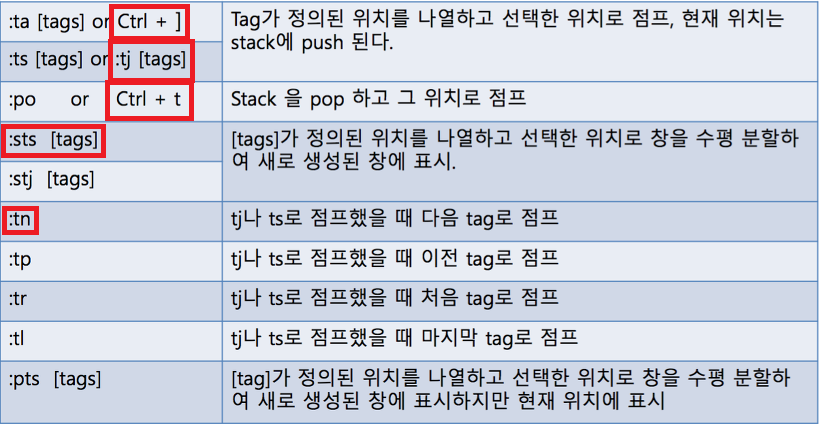
\includegraphics[width=0.8\linewidth]{./figure/command3.png}
\end{figure}
\begin{figure}[h]
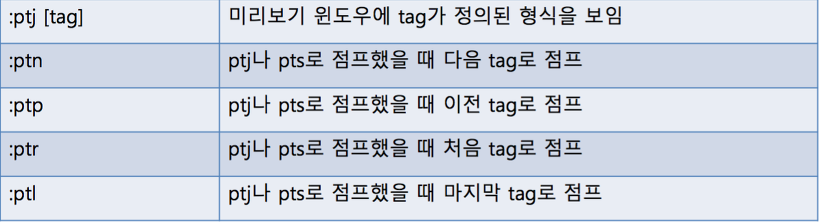
\includegraphics[width=0.8\linewidth]{./figure/command2.png}
\end{figure}
\end{frame}
\section{F2FS 커널수정}
\begin{frame}[containsverbatim,t]
  \frametitle{f2fs-tool 다운로드 및 설치}
\texttt{f2fs-tools}는 리눅스의 파티션을 \texttt{F2FS} 형식으로 포맷할 수 있게 하며,
\begin{mdframed}[backgroundcolor=lightgray,hidealllines=true]
\texttt{\textcolor[rgb]{0,0,0}{\$sudo apt-get install f2fs-tools}}
\end{mdframed}
\bigskip
위 명령어를 통해 설치할 수 있다, 만약 위 명령어대로 설치가 안될 경우
\begin{footnotesize}
\begin{mdframed}[backgroundcolor=lightgray,hidealllines=true]
\texttt{\textcolor[rgb]{0,0,0}{
\$ git clone https://git.kernel.org/pub/scm/linux/kernel/git/jaegeuk/\\
\smallskip
f2fs-tools.git\\
\smallskip
\$ sudo apt-get install uuid-dev pkg-config autoconf libtool libselinux1-dev\\
\smallskip
\$ autoreconf --install\\
\smallskip
\$ ./configure\\
\smallskip
\$ make}}
\end{mdframed}
\end{footnotesize}
\bigskip
명령어를 차례로 입력하여 설치한다.
\end{frame}

\begin{frame}[containsverbatim,t]
  \frametitle{f2fs 커널 수정}
먼저, \texttt{cd}명령어를 통해 \texttt{linux-3.18.1} 폴더로 이동한다.
\begin{mdframed}[backgroundcolor=lightgray,hidealllines=true]
\texttt{\textcolor[rgb]{0,0,0}{\$ cd /'경로'/linux-3.18.1/}}
\end{mdframed}
\bigskip
그 후, 아래 명령어를 통해 미리 컴파일된 `\textbf{원본}' f2fs.ko 파일을 복사한다.
\begin{mdframed}[backgroundcolor=lightgray,hidealllines=true]
\texttt{\textcolor[rgb]{0,0,0}{\$ cp fs/f2fs/f2fs.ko ../modules/f2fs\_ori.ko}}
\end{mdframed}
\bigskip
복사가 완료되면 vi를 실행해 command line 모드로 진입한다.
\begin{mdframed}[backgroundcolor=lightgray,hidealllines=true]
\texttt{\textcolor[rgb]{0,0,0}{\$ vi}}
\end{mdframed}
\bigskip
\end{frame}

\begin{frame}[containsverbatim,t]
  \frametitle{f2fs 커널 수정 - 전역 변수 선언}
아래 명령어처럼 Ctags를 이용해 함수가 정의된 곳(\texttt{segement.h})으로 이동한다.
\begin{mdframed}[backgroundcolor=lightgray,hidealllines=true]
\texttt{\textcolor[rgb]{0,0,0}{:tj nr\_pages\_to\_write}}
\end{mdframed}
\bigskip
\texttt{nr\_pages\_to\_write} 함수 상단에 아래와 같이 전역 변수를 선언한다.
\begin{codedef}
/////////////////////////////////////////////////////////////////////////////
/* 실습용 코드 : 전역 변수들을 선언해준다 */
extern unsigned long long len_user_data;
extern unsigned long long len_fs_write;
/////////////////////////////////////////////////////////////////////////////
static inline long nr_pages_to_write(struct f2fs_sb_info *sbi, int type,
                                        struct writeback_control *wbc)
{
	...
\end{codedef}
\end{frame}


\begin{frame}[containsverbatim,t]
  \frametitle{f2fs 커널 수정 - 전역 변수 초기화}
아래 명령어처럼 Ctags를 이용해 변수가 정의된 곳(\texttt{statement.c})으로 이동한다.
\begin{mdframed}[backgroundcolor=lightgray,hidealllines=true]
\texttt{\textcolor[rgb]{0,0,0}{:tj inmem\_entry\_slab}}
\end{mdframed}
\bigskip
\texttt{inmem\_entry\_slab} 변수 아래에서 선언한 변수의 값을 초기화해준다.
\begin{codedef}
...
static struct kmem_cache *inmem_entry_slab;
/////////////////////////////////////////////////////////////////////////////
/* 실습용 코드 : 선언한 전역 변수들을 초기화 한다 */
unsigned long long len_user_data = 0;  
		// User에서 File System에 쓰여진 데이터의 양
unsigned long long len_fs_write = 0;    
		// File System에서 Block Layer에 쓰여진 데이터의 양
/////////////////////////////////////////////////////////////////////////////
/*
 * __reverse_ffs is copied from include/asm-generic/bitops/__ffs.h since
 * MSB and LSB are reversed in a byte by f2fs_set_bit.
 */
static inline unsigned long __reverse_ffs(unsigned long word)
\end{codedef}
\end{frame}

\begin{frame}[containsverbatim,t]
  \frametitle{f2fs 커널 수정 - User to FS}
아래 명령어처럼 Ctags를 이용해 함수가 정의된 곳으로 이동한다.
\begin{mdframed}[backgroundcolor=lightgray,hidealllines=true]
\texttt{\textcolor[rgb]{0,0,0}{:tj f2fs\_write\_begin}}
\end{mdframed}
\bigskip
\texttt{f2fs\_write\_begin} 함수 내부에 아래와 같이 코드를 입력한다.
\begin{codedef}
static int f2fs_write_begin(struct file *file, struct address_space *mapping,
                loff_t pos, unsigned len, unsigned flags,
                struct page **pagep, void **fsdata)
{
        ...
        trace_f2fs_write_begin(inode, pos, len, flags);
//////////////////////////////////////////////////////////////////////////       
/* 실습용 코드 : User영역에서 File system에 쓰는 Data의 크기를 기록 */
        len_user_data += len;
//////////////////////////////////////////////////////////////////////////
        f2fs_balance_fs(sbi);
        ...
}
\end{codedef}
\end{frame}

\begin{frame}[containsverbatim,t]
  \frametitle{f2fs 커널 수정 - FS to Block Layer 1}
아래 명령어처럼 Ctags를 이용해 함수가 정의된 곳으로 이동한다.
\begin{mdframed}[backgroundcolor=lightgray,hidealllines=true]
\texttt{\textcolor[rgb]{0,0,0}{:tj \_\_submit\_merged\_bio}}
\end{mdframed}
\bigskip
\texttt{\_\_submit\_merged\_bio} 함수 내부에 아래와 같이 코드를 입력한다.
\begin{codedef}

static void __submit_merged_bio(struct f2fs_bio_info *io)
{
        ...
//////////////////////////////////////////////////////////////////////////       
/* 실습용 코드 : File system에서 Block Layer에 쓰는 Data의 크기를 기록 */
        if(!is_read_io(fio->rw)){
                len_fs_write += io->bio->bi_vcnt * 4096;
        }
//////////////////////////////////////////////////////////////////////////    
        io->bio = NULL;
}
\end{codedef}
\end{frame}

\begin{frame}[containsverbatim,t]
  \frametitle{f2fs 커널 수정 - FS to Block Layer 2}
아래 명령어처럼 Ctags를 이용해 함수가 정의된 곳으로 이동한다.
\begin{mdframed}[backgroundcolor=lightgray,hidealllines=true]
\texttt{\textcolor[rgb]{0,0,0}{:tj f2fs\_submit\_page\_bio}}
\end{mdframed}
\bigskip
\texttt{f2fs\_submit\_page\_bio} 함수 내부에 아래와 같이 코드를 입력한다.
\begin{codedef}

int f2fs_submit_page_bio(struct f2fs_sb_info *sbi, struct page *page,
                                        block_t blk_addr, int rw)
{
        ...
//////////////////////////////////////////////////////////////////////////       
/* 실습용 코드 : File system에서 Block Layer에 쓰는 Data의 크기를 기록 */
        if(!is_read_io(rw)){
                len_fs_write += bio->bi_vcnt * 4096;
        }
//////////////////////////////////////////////////////////////////////////    
        submit_bio(rw, bio);
        return 0;
}
\end{codedef}
\end{frame}

\begin{frame}[containsverbatim,t]
  \frametitle{f2fs 커널 수정 - Data의 양 표시}
아래 명령어처럼 Ctags를 이용해 함수가 정의된 곳으로 이동한다.
\begin{mdframed}[backgroundcolor=lightgray,hidealllines=true]
\texttt{\textcolor[rgb]{0,0,0}{:tj stat\_show}}
\end{mdframed}
\bigskip
\texttt{stat\_show} 함수 내부에 아래와 같이 코드를 입력한다.
\begin{codedef}
static int stat_show(struct seq_file *s, void *v)
{
        ...
        seq_printf(s, "(OverProv:%d Resv:%d)]\n\n", 
                           si->overp_segs, si->rsvd_segs);
/////////////////////////////////////////////////////////////////////////////
/* 실습용 코드 : User영역, File System, Block Layer 간 쓰여진 data의 양 표시 */
        seq_printf(s, "Buffered Write Information :\n");
        seq_printf(s, "  - User to FS: %llu bytes\n", len_user_data);
        seq_printf(s, "  - FS to Block Layer: %llu bytes\n\n", len_fs_write);
/////////////////////////////////////////////////////////////////////////////
        ...
}
\end{codedef}
\end{frame}

\begin{frame}[containsverbatim,t]
  \frametitle{f2fs 모듈 컴파일}
\texttt{cd}명령어를 통해 다시 \texttt{linux-3.18.1} 폴더로 이동한다.
\begin{mdframed}[backgroundcolor=lightgray,hidealllines=true]
\texttt{\textcolor[rgb]{0,0,0}{\$ cd /'경로'/linux-3.18.1/}}
\end{mdframed}
\bigskip
그 후, 아래 명령어를 통해 수정된 f2fs 커널의 모듈을 컴파일한다.
\begin{mdframed}[backgroundcolor=lightgray,hidealllines=true]
\texttt{\textcolor[rgb]{0,0,0}{\$ make modules}}
\end{mdframed}
\bigskip
컴파일이 완료되면 `\textbf{새로운}' f2fs.ko 파일을 복사한다.
\begin{mdframed}[backgroundcolor=lightgray,hidealllines=true]
\texttt{\textcolor[rgb]{0,0,0}{\$ cp fs/f2fs/f2fs.ko ../modules/f2fs\_new.ko}}
\end{mdframed}
\bigskip
\end{frame}
\section{F2FS 실습}
\begin{frame}[containsverbatim,t]
  \frametitle{f2fs 모듈 적재(Load)}
\texttt{rmmod}명령어를 통해 f2fs 모듈을 제거한다.
\begin{mdframed}[backgroundcolor=lightgray,hidealllines=true]
\texttt{\textcolor[rgb]{0,0,0}{\$ sudo rmmod f2fs}}
\end{mdframed}
\bigskip
만약 F2FS 모듈이 없는 경우에는 아래와 같이
\begin{mdframed}[backgroundcolor=lightgray,hidealllines=true]
\texttt{\textcolor[rgb]{0,0,0}{'ERROR: Module f2fs does not exist in /proc/modules'}}
\end{mdframed}
\bigskip
경고문이 출력된다.\\ 
모듈이 제거 후 \texttt{f2fs\_ori.ko}, \texttt{f2fs\_new.ko}파일이 있는 폴더로 이동 한다.
\begin{mdframed}[backgroundcolor=lightgray,hidealllines=true]
\texttt{\textcolor[rgb]{0,0,0}{\$ cd ../modules}}
\end{mdframed}
\bigskip
모듈은 아래와 같이 \texttt{insmod}명령어로 적재(Load) 할 수 있다.
\begin{mdframed}[backgroundcolor=lightgray,hidealllines=true]
\texttt{\textcolor[rgb]{0,0,0}{\$ sudo insmod f2fs\_new.ko}}
\end{mdframed}
\bigskip
\end{frame}

\begin{frame}[containsverbatim,t]
  \frametitle{파티션 F2FS 포맷}
\texttt{cd}명령어를 통해 codes 폴더로 이동한다.
\begin{mdframed}[backgroundcolor=lightgray,hidealllines=true]
\texttt{\textcolor[rgb]{0,0,0}{\$ cd ../codes}}
\end{mdframed}
\bigskip
실험에 사용할 파티션은 시스템이 사용하는 파티션이 아닌 다른 파티션을 사용한다. 여기서는 /dev/sdb1을 사용하도록 한다. 

codes폴더 내부의 \texttt{mkfs.f2fs} 파일로 /dev/sdb1 파티션을 포맷한다.
\begin{mdframed}[backgroundcolor=lightgray,hidealllines=true]
\texttt{\textcolor[rgb]{0,0,0}{\$ sudo ./mkfs.f2fs \-l mnt /dev/sdb1}}
\end{mdframed}
\bigskip
성공적으로 포맷 시 아래 문구가 출력된다.
\begin{mdframed}[backgroundcolor=lightgray,hidealllines=true]
\texttt{\textcolor[rgb]{0,0,0}{Info: format successful}}
\end{mdframed}
\bigskip
\end{frame}

\begin{frame}[containsverbatim,t]
  \frametitle{F2FS 파일시스템 마운트}
\begin{footnotesize}
F2FS으로 포맷된 파티션을 다음과 같은 명령어로 마운트시킨다.
\begin{mdframed}[backgroundcolor=lightgray,hidealllines=true]
\texttt{\textcolor[rgb]{0,0,0}{\$ sudo mount -t f2fs /dev/sdb1 ./mnt/}}
\end{mdframed}
\bigskip
폴더를 마운트 한 후 \texttt{F2FS}의 상태를 보여주는
\begin{mdframed}[backgroundcolor=lightgray,hidealllines=true]
\texttt{\textcolor[rgb]{0,0,0}{\$ sudo cat /sys/kernel/debug/f2fs/status}}
\end{mdframed}
\bigskip
명령어를 입력하여 아래와 같은 화면이 출력되면,\\
\medskip
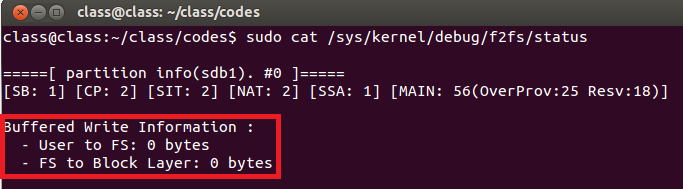
\includegraphics[width=0.8\linewidth]{./figure/f2fsstatus.png}
\\
\texttt{F2FS} 환경에서 File System 및 Block Layer에 쓰여지는 Data의 양을 확인할 수 있다.
\end{footnotesize}
\end{frame}

\begin{frame}[containsverbatim,t]
  \frametitle{F2FS 파일시스템 실습 1}
\texttt{F2FS}의 상태를 보여주는 아래 명령어를 이용하여 
\begin{mdframed}[backgroundcolor=lightgray,hidealllines=true]
\texttt{\textcolor[rgb]{0,0,0}{\$ sudo cat /sys/kernel/debug/f2fs/status}}
\end{mdframed}
\bigskip
\texttt{F2FS} 마운트 폴더인 mnt 내부에서 다음과 같은 명령어들을 실행하며 Data 양의 변화를 살펴보자.
\begin{mdframed}[backgroundcolor=lightgray,hidealllines=true]
\texttt{\textcolor[rgb]{0,0,0}{\$ sudo mkdir test\\
\$ sudo cat /proc/modules >> a.txt\\
\$ sudo rm -r test\\
\$ sudo cp a.txt b.txt\\
\$ sudo rm a.txt\\
\$ sudo rm b.txt}}
\end{mdframed}
\end{frame}

\begin{frame}[containsverbatim,t]
  \frametitle{F2FS 파일시스템 실습 2}
\texttt{F2FS}의 상태를 보여주는 아래 명령어를 이용하여 
\begin{mdframed}[backgroundcolor=lightgray,hidealllines=true]
\texttt{\textcolor[rgb]{0,0,0}{\$ sudo cat /sys/kernel/debug/f2fs/status}}
\end{mdframed}
\bigskip
\texttt{F2FS} 마운트 폴더인 mnt 내부에 테스트 프로그램인 `\texttt{sysp}'를 실행한 후 Data 양의 변화를 살펴보자. 
\begin{mdframed}[backgroundcolor=lightgray,hidealllines=true]
\texttt{\textcolor[rgb]{0,0,0}{\$ cd mnt\\
\$ cp ../codes/sysp .\\
\$ sudo ./sysp}}
\end{mdframed}
\begin{footnotesize}
\medskip
\begin{block}{
\begin{scriptsize}
sysp 테스트 프로그램
\end{scriptsize}
}\medskip
\texttt{sysp} 테스트 프로그램은 \texttt{f\_0.txt}부터 \texttt{f\_9.txt}까지 총 10개의 \texttt{3Kbyte} 파일을 Buffered write한 후,마지막 \texttt{f\_9.txt} 파일에 대해서만 \texttt{fsync}() 함수를 실행하는 프로그램이다. 
\end{block}
\end{footnotesize}
\end{frame}

\end{document}
